

%%%%%%%%%%%%%%%%%%%%%%%%%%%%%%%%%%%%%%%%%%%%%%%%%%%%%%%%%%%%%%%%%%%%%%%%%%%%%%%%
%%%%%%%%%%%%%%%%%%%%%%%%%%%%%%%%%%%%%%%%%%%%%%%%%%%%%%%%%%%%%%%%%%%%%%%%%%%%%%%%
\section{\textcolor{red}{Dançar no ritmo}}
\label{subsec:dancaritmo}
\index{Musicalidade!Dançar no ritmo}
 Dançar usando o \hyperref[sec:pos:Ritmo]{\textbf{ritmo}},
é um estágio intermediario de nosso percorrido na musicalidade;
para atingir a competência neste estagio, 
devemos aprender a aproveitar todas as informações encontradas 
no ritmo, provenientes de alguma linha melódica, acompanhamento ou da música como um todo.

No modo mais simples ou cru, poderíamos pensar no ritmo,
como um conjunto de \hyperref[sec:figurasmusicais]{\textbf{figuras musicais}} 
colocadas uma apos de outra, 
e explorar o ritmo, figura a figura musical. % este \hyperref[sec:elementosmusica]{\textbf{elemento da música}}.
Porem, ao igual que quando escutamos um discurso,
sabemos que este em essência é um conjunto de letras colocadas uma apos outra,
e poderíamos entender-lho estudando-o desde essa perspetiva;
para nós seres humanos, 
muitas vezes é mais fácil pensar sempre em macro que em micro,
ou seja em estruturas maiores como palavras ou frases, perguntas, respostas ou ordens, etc. 
De modo que nosso cérebro, em muitos casos, 
já está adaptado com soluciones prontas para atender estes problemas.

Antes de passar a descrever estruturas maiores, 
é importante lembrar elementos menores que podem ser aproveitadas na música.
Primeiro devemos lembrar que existem 4 \hyperref[sec:carateristasom]{\textbf{características do som}},
estas são: 
\begin{inparaitem}
\item o tom, 
\item a duração, 
\item o timbre e 
\item a intensidade.
\end{inparaitem}
Destas quatro só o tom não vai ser aproveitado se dançamos no ritmo;
porem podemos usar o timbre e a intensidade do som para mudar nossas 
\hyperref[sec:musicalidade:dinamicas]{\textbf{dinâmicas do movimento}};
já a duração poderia ser usada dançando o ritmo figura musical por figura,
movimentando-nos atrelados a esse elemento.

Por outro lado, a nível macro, temos  motivos e frases rítmicas,
que poderíamos aproveitar seguindo elas ou interpretando-as, 
com suas obvias consequência como o melhor aproveitamento das pausas, 
como nos finais de frase musical ou nos ``breaks'' da música,
ou mudanças de movimentos na mudança de frase.

%Assim, quando percebemos o ritmo numa música, 
%podemos sim usar este elemento da música, figura a figura; 
%porem, devemos lembrar que temos outros aspectos do ritmo,
%agrupadas em estruturas maiores e menos evidentes que podemos aproveitar.


\begin{example}[dançando no ritmo seguindo as figuras musicais:]
\label{ex:dancaritmo1}
Imaginemos que temos decidido executar nossos movimentos (ex: pisadas, ou movimentos de ombros, cabeça quadril, etc.),
seguindo o ritmo de uma camada numa peça musical.
Nesse caso, uma possível alternativa para dançar no ritmo, 
seria movimentar nosso corpo seguindo uma a uma as figuras musicais.

Assumindo esta  consideração criativa para nossos movimentos, 
podemos usar a melodia ``Lamento e consolo'' (ver Figura \ref{fig:lamento-e-consolo}),
para dançar no ritmo, 
de modo que nossos movimentos seriam executados como indica a Figura \ref{fig:lamentoconsoloritmo1}.
A melodia a dançar está representada por um ``bandolim'',
e as ``claves'' representam o ritmo que seguem nossos movimentos;
nesse caso foram escolhidos pisadas, como movimentos de exemplo.
É fácil perceber, nessa representação, 
como nossos movimentos estão atrelados ao ritmo na música,
e não a outras informações como o tom das notas musicais.
\end{example}
\begin{sidewaysfigure}
    \centering
    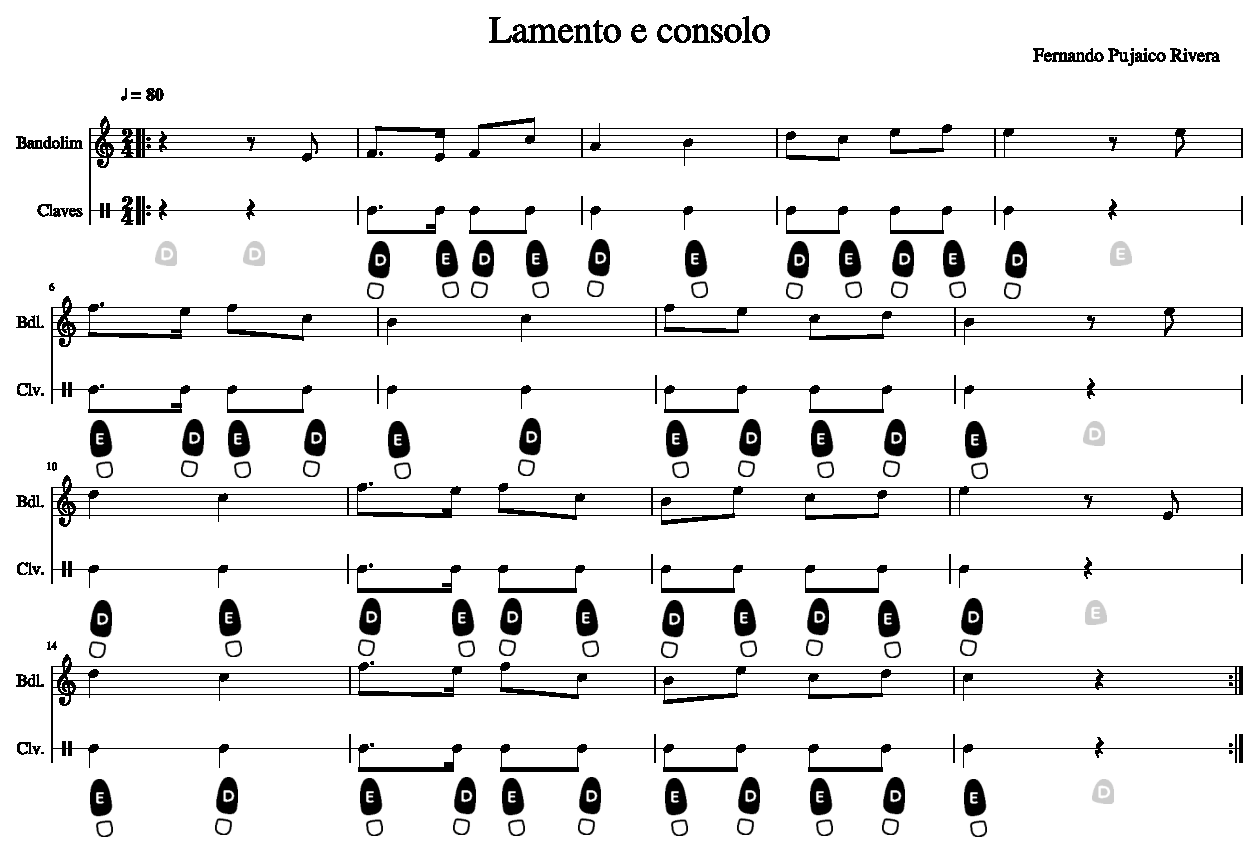
\includegraphics[width=\textwidth]{chapters/cap-musicalidade-tecnica/lamento-e-consolo-clave-ritmo-1.eps}
    \caption{Música dançada no ritmo.}
    \label{fig:lamentoconsoloritmo1}
\end{sidewaysfigure}


No quesito de dançar no ritmo, muitos professores e autores propuseram diferentes jeitos de aproveitar o ritmo; 
por exemplo, o dançarino e instrutor ``Andrew Sutton'', 
no seu blog sobre dança ``danceninjas'',
menciona na sua visão, alguns aspectos do ritmo que podem ser aproveitados \cite{AndrewSuttonRitmo1};
a seguir mostramos uma descrição destes conceitos.  
\begin{itemize}
%%%%%
\item Acertando a velocidade da dança em relação ao \hyperref[sec:Andamento]{\textbf{andamento}}:
Como já foi visto na Seção \ref{sec:Andamento},
o andamento é uma caraterística importante na música,
pois define o grau de lentidão ou rapidez ao executar,
uma peça musical. 
Dado que as figuras musicais, usadas para descrever um ritmo, 
só tem uma duração com valor relativo entre elas,
conhecer o andamento; é dizer, conhecer quantas batidas por minuto (BPM) tem cada figura musical,
nos ajudará a acertar qual deve ser a velocidade meia de nossa dança,
e predizer corretamente qual será a duração mínima e máxima da seguinte figura musical executada.
\begin{example}
Podemos perceber esta diferencia entre os andamentos, 
ao escutar a música ``Delírios de amor'' interpretada por ``Alcione'', 
de andamento lento, 
quanto comparado com a música ``vanerão sambado'' interpretado pelo grupo ``Os serranos'', 
com um andamento de maior rapidez.
De modo que para nos é evidente que em media nossos movimentos serão mais lentos,
no primeiro caso que no segundo.
\end{example}
%%%%%
\item Melhorando nosso \hyperref[sec:dancetimming]{\textbf{timing}}:
Este ponto já foi abordado na Seção \ref{sec:dancetimming},
onde se indica que ter a capacidade de ter o peso bem definido,
ao inicio de cada \hyperref[sec:TemposCoreograficos]{\textbf{tempo coreográfico}}, 
é muito importante esteticamente para projetar clareza em nossos movimentos,
e tecnicamente para poder ter o tempo completo entre movimentos consecutivos,
para poder executar \hyperref[sec:musicalidade:dinamicas]{\textbf{dinâmicas}}.
%%%%%
\item Seguindo as \hyperref[sec:figurasmusicais]{\textbf{figuras musicais}}:
A forma mais evidente de aproveitar o ritmo, 
é seguindo as figuras musicais com nossos movimentos;
assim, nesta tarefa podemos separar os ritmos percebidos em dois casos:
\begin{itemize} 
\item No primeiro, o ritmo que escolhemos tem uma caraterista cíclica ou regular,
aos quais denominaremos aqui como ritmos simples; podemos ver exemplos de ritmos simples,
no acompanhamento de uma linha melódica, 
pois geralmente estes repetem de forma cíclica uma frase rítmica curta.
\item No segundo caso, temos  ritmos compostos por figuras musicais,
com uma caraterista não cíclica num período longo de tempo; 
chamaremos a estos como ritmos complexos;
estes casos são vistos facilmente no ritmo da linha melódica principal de uma composição musical.
\end{itemize}
Mesmo que sejam dados exemplos específicos, 
indicando onde comumente poderemos achar ritmos simples e complexos;
na prática poderemos achar estes ritmos em qualquer camada de uma música,
ou pelo menos em uma seção dela; 
pois seus usos estão limitados só pela criatividade do compositor.
%%%%%
\item Usando \hyperref[sec:musicalidade:dinamicas]{\textbf{dinâmicas}} no ritmo: 
Uma forma de dar variedade e textura a nossos movimentos, 
é usando dinâmicas; este tema já foi tratado na Seção \ref{sec:musicalidade:dinamicas},
onde também estudamos os fatores do movimento.

Assim, algumas opções para trabalhar nosso ritmo usando dinâmicas, seriam:
\begin{itemize}
\item Aproveitar o \hyperref[sec:pos:timbre]{\textbf{timbre}} dos instrumentos que geram o ritmo,
para modelar nossas dinâmicas.
\begin{example}[Bumbo vs. pandeiro:]
quando seguimos  o ritmo executado pelo bumbo,
podemos fazer movimentos mais pesados ou com uma aparência de dançar num lugar com gravidade aumentada,
porem se o mesmo ritmo fosse executado por um pandeiro,
nossos movimento,
poderiam dar uma aparência de agilidade, 
como de algo que se movimenta ligeiramente.
\end{example}
\item Podemos também escolher uma porção do ritmo, como um motivo rítmico,
 ou o que consideremos ideias rítmica curtas,
é interpretar-lho com nossos movimentos seguindo alguma dinâmica.
\begin{example}[Usando motivos rítmicos:]
Damos passos pisando só a última figura musical de um motivo rítmico,
de modo que o movimento, para dar esse passo, pode ser rápido ou lento,
dependendo do juízo que façamos sobre o resto de figuras musicais do motivo.
Onde por exemplo, se são muitas figuras musicais de duração curta, 
faremos um movimento rápido para pisar a última figura;
e se as figuras musicais são poucas e de longa duração faremos um movimento lento.
\end{example}
\end{itemize}
\end{itemize}

